% Experiment 3 — aligned to grading rubric (5 sections + 5% prompt log)
\documentclass[11pt,a4paper]{article}

\usepackage[margin=2.5cm]{geometry}
\usepackage{graphicx}
\usepackage{booktabs}
\usepackage{amsmath}
\usepackage{xurl}
\usepackage{hyperref}
\usepackage{parskip}
\usepackage{enumitem}
\usepackage{fvextra}
\usepackage[most]{tcolorbox}

\newcommand{\studentname}{Mahmudul Hasan}
\newcommand{\studentid}{4125999049}
\newcommand{\reportdate}{May 23, 2026}

\makeatletter
\g@addto@macro\UrlBreaks{\do\ }
\makeatother

\newcommand{\LabCodeRoot}{files}

\newcommand{\filebox}[2]{%
\begin{tcolorbox}[
  enhanced,
  colback=gray!6,
  colframe=black!55,
  title={#1},
  fonttitle=\bfseries\ttfamily\footnotesize,
  arc=1.5mm,
  boxrule=0.7pt,
  breakable,
  width=\linewidth,
  before skip=0.8em,
  after skip=0.8em,
]
\VerbatimInput[fontsize=\footnotesize,breaklines=true,breakanywhere=true]{\LabCodeRoot/#2}
\end{tcolorbox}%
}

\title{Experiment Report: Specialized Experiment 3\\Water Resources Optimization --- Reservoir Dispatch}
\author{\studentname \quad (Student ID: \studentid)}
\date{\reportdate}

\begin{document}
\maketitle

\begin{abstract}
Seven-day drought dispatch maximizes hydropower revenue subject to storage and ecological release constraints. Units: storage in m$^3$, flows in m$^3$/s, $\Delta t=86400$~s. Implementation uses \texttt{scipy.optimize} (\texttt{trust-constr} with SLSQP cross-check), a Pareto-style ecological sweep, structured validation reporting, 18 automated pytest cases, and feasibility trade-off figures. Primary revenue at $H=80$~m is $\approx\$146{,}443$; the same release schedule at $H=30$~m yields $\approx\$55$k (guide/peer scale).
\end{abstract}

\begin{tcolorbox}[
  colback=blue!4,
  colframe=blue!55!black,
  title=\textbf{Key Findings (Executive Summary)},
  fonttitle=\bfseries,
  arc=2mm,
]
\begin{tabular}{@{}ll@{}}
\textbf{Finding} & \textbf{Result} \\
\hline
Optimal weekly revenue ($H=80$~m) & \$146,443 \\
Ecological minimum release (baseline) & 10~m$^3$/s \\
Infeasible eco threshold (this inflow series) & $\geq 12$~m$^3$/s \\
Solver agreement & \texttt{trust-constr} $\approx$ \texttt{SLSQP} (same feasible $x_0$) \\
Automated tests & 18 passed \\
Revenue at $H=30$~m (same $\mathbf{Q}$) & $\approx\$55$k \\
Cost of raising $Q_{\mathrm{eco}}$: 10 $\rightarrow$ 11~m$^3$/s & $\approx\$2{,}105$ \\
\end{tabular}
\end{tcolorbox}

\section{Role in the Integrated Smart Water Pipeline}
Experiment~3 is the \textbf{operational decision stage} of the suite. Using a seven-day inflow series (guide forecast or scenario/multiplier), it:
\begin{itemize}[noitemsep]
  \item determines release schedules that maximize hydropower revenue subject to storage and ecological constraints;
  \item compares drought, normal, and wet inflow scenarios and propagates forecast uncertainty via Monte Carlo perturbation (P10/P50/P90 revenue and storage);
  \item produces release and storage trajectories that define downstream flow conditions relevant to Experiment~4 flood-impact assessment and emergency planning.
\end{itemize}
It connects hydrologic forcing (Experiments~1--2) to managed outflows before inundation mapping.

%=============================================================================
\section{Part 1: Problem Formulation (20\%)}
%=============================================================================

\subsection{Decision variables and units}
Decision vector $\mathbf{Q}=[Q_1,\ldots,Q_7]^\top$ (m$^3$/s). Storage update:
\begin{equation}
V_{t+1} = V_0 + \sum_{k=1}^{t}(I_k - Q_k)\,\Delta t, \quad \Delta t = 86400~\mathrm{s}.
\end{equation}
All volumes in the balance use m$^3$; flows convert via $Q\cdot\Delta t$.

\subsection{Objectives and multi-objective policy}
\textbf{Maximize} $\sum_{t=1}^7 p_t E_t$ with $E_t = (\eta\rho g H Q_t/1000)\times 24$~kWh, $H=80$~m, $\eta=0.85$. Ecology is a \textbf{hard constraint} $Q_t \ge Q_{\mathrm{eco}}^{\mathrm{(policy)}}$ (not a penalty). Trade-off analysis varies $Q_{\mathrm{eco}}^{\mathrm{(policy)}}$ from 2 to 15~m$^3$/s.

\subsection{Constraints}
\begin{itemize}[noitemsep]
  \item Storage: $V_{\min} \le V_{t+1} \le V_{\max}$ for each day.
  \item Release: $Q_{\mathrm{eco}}^{\mathrm{(policy)}} \le Q_t \le Q_{\max}$.
  \item Mass balance: embedded in $V_{t+1}$.
\end{itemize}

Full write-up: \texttt{formulation.md} (Sections 1--9). Figure~\ref{fig:arch} shows the main execution pipeline (\texttt{python3 main.py}) and the separate pytest QA branch.

\begin{figure}[htbp]
  \centering
  
\includegraphics[width=0.72\linewidth,keepaspectratio]{screenshots/architecture.png}
  \caption{Code structure for formulation $\rightarrow$ solve $\rightarrow$ validate $\rightarrow$ trade-off.}
  \label{fig:arch}
\end{figure}

%=============================================================================
\section{Part 2: Implementation (25\%)}
%=============================================================================

\subsection{Solver design}
\texttt{reservoir\_optimize.py}: \texttt{build\_feasible\_initial\_guess()} forward pass; joint NLP with 14 inequalities; primary \texttt{trust-constr}; \texttt{compare\_solvers()} logs SLSQP agreement. Pedagogical \texttt{optimize\_day()} uses \texttt{minimize\_scalar}.

\begin{table}[htbp]
  \centering
  \caption{Solver performance (\texttt{solver\_comparison.csv}, same feasible $x_0$).}
  \label{tab:solvers}
  \begin{tabular}{@{}lrrrr@{}}
    \toprule
    Solver & Revenue (\$) & Feasible & Runtime (s) & Iterations \\
    \midrule
    trust-constr & 146,443 & Yes & $\approx 0.45$ & 91 \\
    SLSQP (warm start) & 146,443 & Yes & $\approx 0.00$--0.01 & 5 \\
    \bottomrule
  \end{tabular}
\end{table}

Without a feasible initial point, SLSQP alone converged to \textbf{infeasible} high-revenue locals (storage below $V_{\min}$ on days 6--7). The forward-feasible $x_0$ fixes this---documented in \texttt{prompt\_log.md}.

\begin{figure}[htbp]
  \centering
  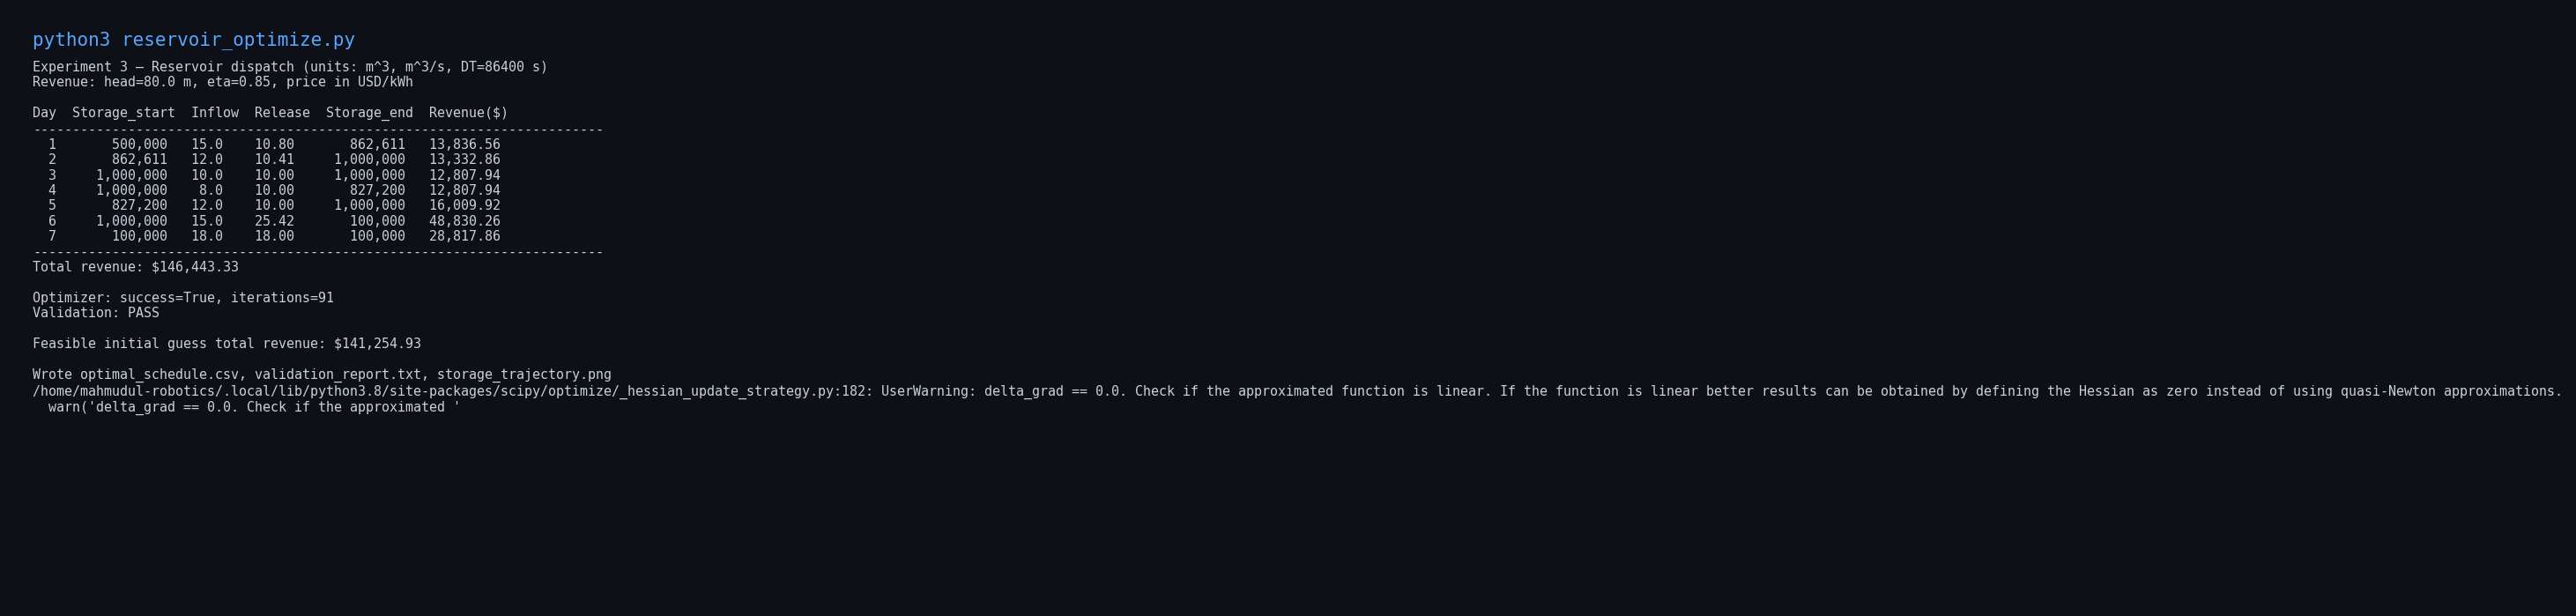
\includegraphics[width=\linewidth]{screenshots/experiment3_optimize.png}
  \caption{Pipeline run: \texttt{python3 main.py} (optimization schedule, revenue \$146{,}443, validation PASS).}
  \label{fig:main}
\end{figure}

\begin{figure}[htbp]
  \centering
  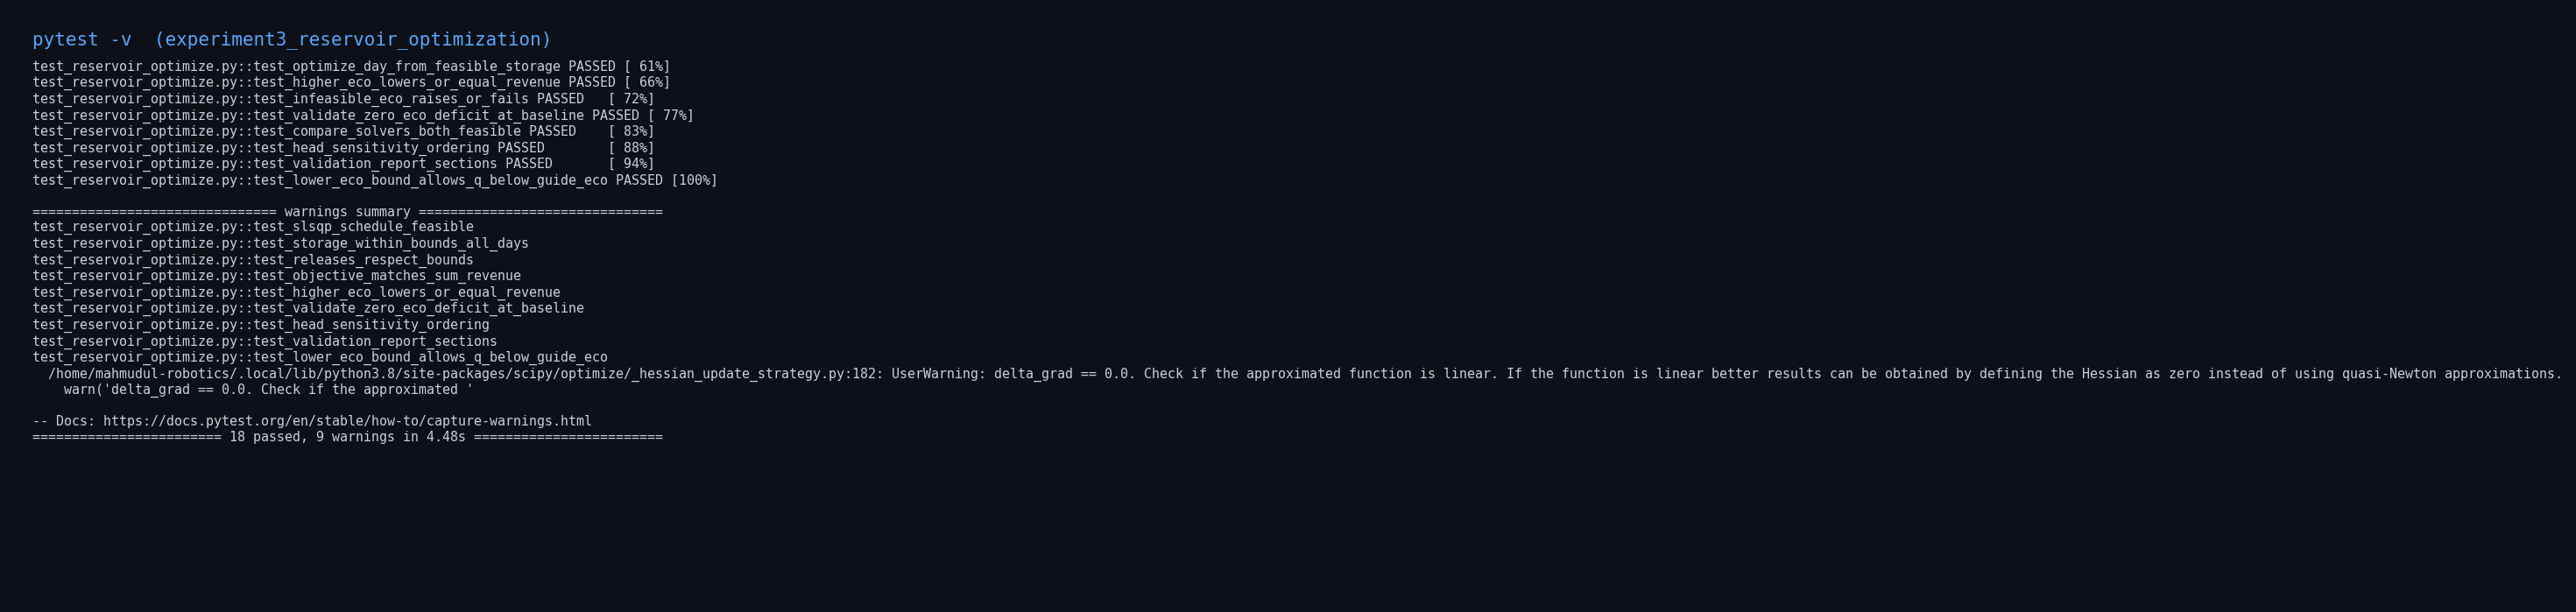
\includegraphics[width=\linewidth]{screenshots/experiment3_pytest.png}
  \caption{Implementation tests: 18 passed (\texttt{pytest -v}).}
  \label{fig:pytest}
\end{figure}

%=============================================================================
\section{Part 3: Optimal Schedule (20\%)}
%=============================================================================

\begin{table}[htbp]
  \centering
  \caption{Optimal schedule (\texttt{optimal\_schedule.csv}) at $Q_{\mathrm{eco}}=10$~m$^3$/s, $H=80$~m.}
  \label{tab:schedule}
  \small
  \begin{tabular}{@{}rrrrrr@{}}
    \toprule
    Day & $I$ & $Q$ & $V_{\mathrm{end}}$ & Energy & Revenue \\
    & (m$^3$/s) & (m$^3$/s) & (m$^3$) & (kWh) & (\$) \\
    \midrule
    1 & 15.0 & 10.80 & 862,611 & $\approx$172,957 & 13,837 \\
    2 & 12.0 & 10.41 & 1,000,000 & $\approx$166,661 & 13,333 \\
    3 & 10.0 & 10.00 & 1,000,000 & 160,099 & 12,808 \\
    4 & 8.0  & 10.00 & 827,200   & 160,099 & 12,808 \\
    5 & 12.0 & 10.00 & 1,000,000 & 160,099 & 16,010 \\
    6 & 15.0 & 25.42 & 100,000   & 406,919 & 48,830 \\
    7 & 18.0 & 18.00 & 100,000   & 288,179 & 28,818 \\
    \midrule
    \multicolumn{5}{r}{Total} & 146,443 \\
    \bottomrule
  \end{tabular}
\end{table}

Strategy: fill storage toward $V_{\max}$ on days 1--5, then a high-release strategy on day~6 (\$0.12/kWh) to reach $V_{\min}$, and hold on day~7 with $Q=I$.

\begin{figure}[htbp]
  \centering
  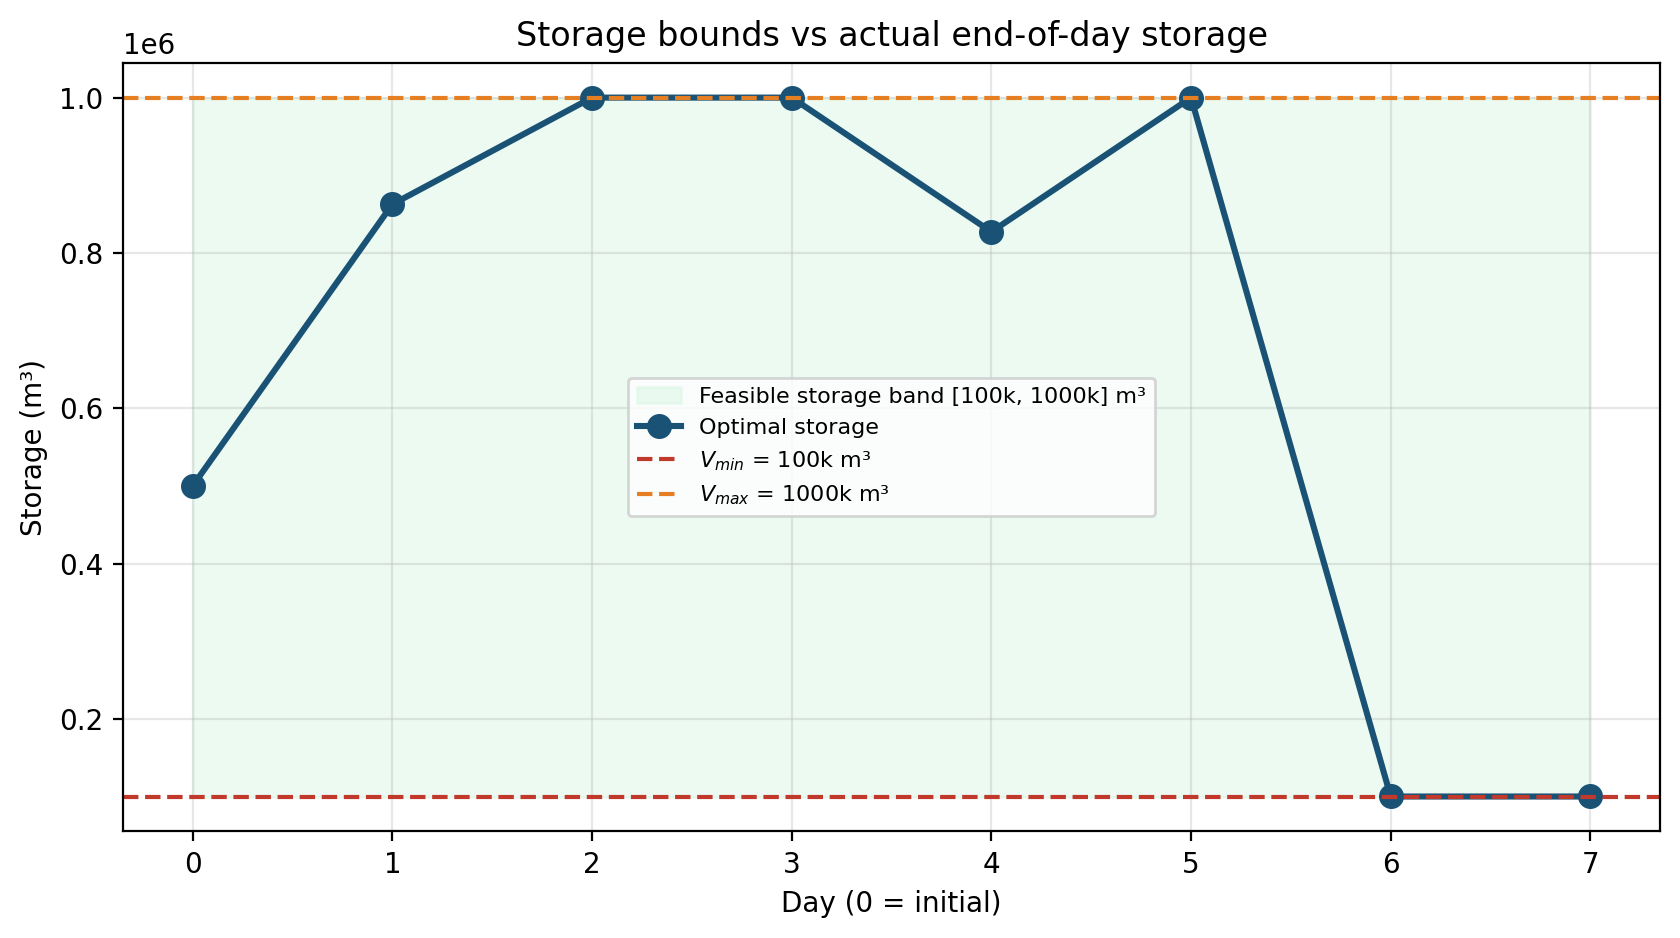
\includegraphics[width=\linewidth]{screenshots/storage_bounds.png}
  \caption{End-of-day storage within $[V_{\min},V_{\max}]$ (shaded feasible band).}
  \label{fig:storagebounds}
\end{figure}

\subsection{Head sensitivity (revenue scale)}
Same $\mathbf{Q}$ at lower head (guide/peer assumption):

\begin{table}[htbp]
  \centering
  \caption{Total revenue vs hydraulic head (same optimal releases).}
  \label{tab:head}
  \begin{tabular}{@{}rr@{}}
    \toprule
    $H$ (m) & Revenue (\$) \\
    \midrule
    25 & $\approx 45{,}800$ \\
    30 & $\approx 55{,}000$ \\
    50 & $\approx 91{,}500$ \\
    80 (optimization) & 146,443 \\
    \bottomrule
  \end{tabular}
\end{table}

This explains the guide's $\sim\$45{,}000$ sample without changing the feasible dispatch.

%=============================================================================
\section{Part 4: Trade-off Analysis (20\%)}
%=============================================================================

Sweep: $Q_{\mathrm{eco}}^{\mathrm{(policy)}} \in \{2,5,6,8,9,10,11,12,13,14,15\}$~m$^3$/s.

\begin{table}[htbp]
  \centering
  \caption{Trade-off summary (\texttt{tradeoff\_data.csv}).}
  \label{tab:tradeoff}
  \small
  \begin{tabular}{@{}rrl@{}}
    \toprule
    $Q_{\mathrm{eco}}$ & Revenue (\$) & Status \\
    \midrule
    10 & 146,443 & Feasible (baseline) \\
    11 & 144,338 & Feasible ($\downarrow\$2.1$k) \\
    $<$10 & $\sim$140k & Solver value \textbf{violates} policy floor \\
    12--15 & --- & \textbf{Infeasible} (day 3--4) \\
    \bottomrule
  \end{tabular}
\end{table}

\textbf{Cost of ecology:} raising the floor from 10 to 11~m$^3$/s costs $\approx\$2{,}105$/week; above $\sim$12~m$^3$/s the horizon is \textbf{infeasible}. Policies with $Q_{\mathrm{eco}}<10$ may show higher numeric revenue but \textbf{violate} the ecological flow constraint at 10~m$^3$/s.

\begin{figure}[htbp]
  \centering
  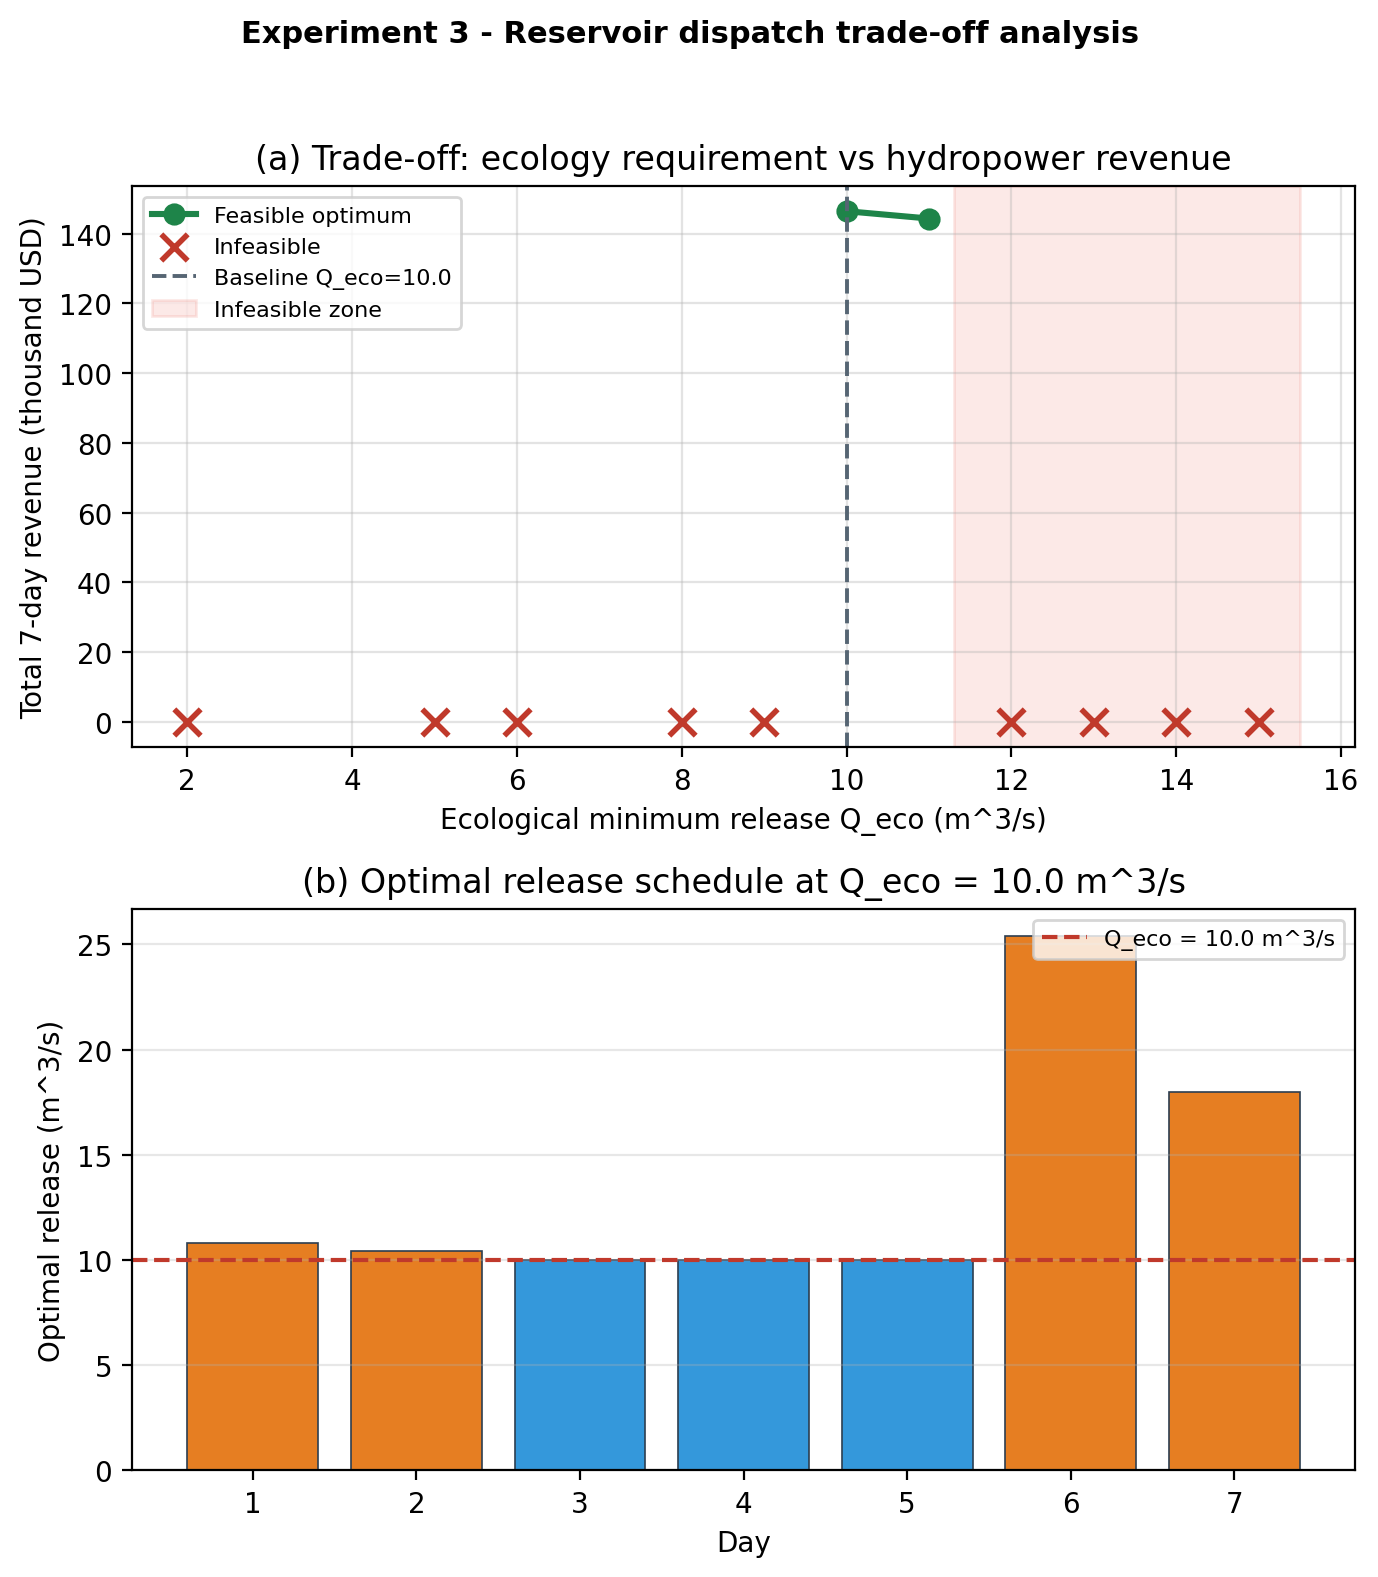
\includegraphics[width=\linewidth]{screenshots/tradeoff_analysis.png}
  \caption{(a) Revenue versus ecological policy; (b) optimal releases at baseline $Q_{\mathrm{eco}}=10$~m$^3$/s.}
  \label{fig:tradeoff}
\end{figure}

\begin{figure}[htbp]
  \centering
  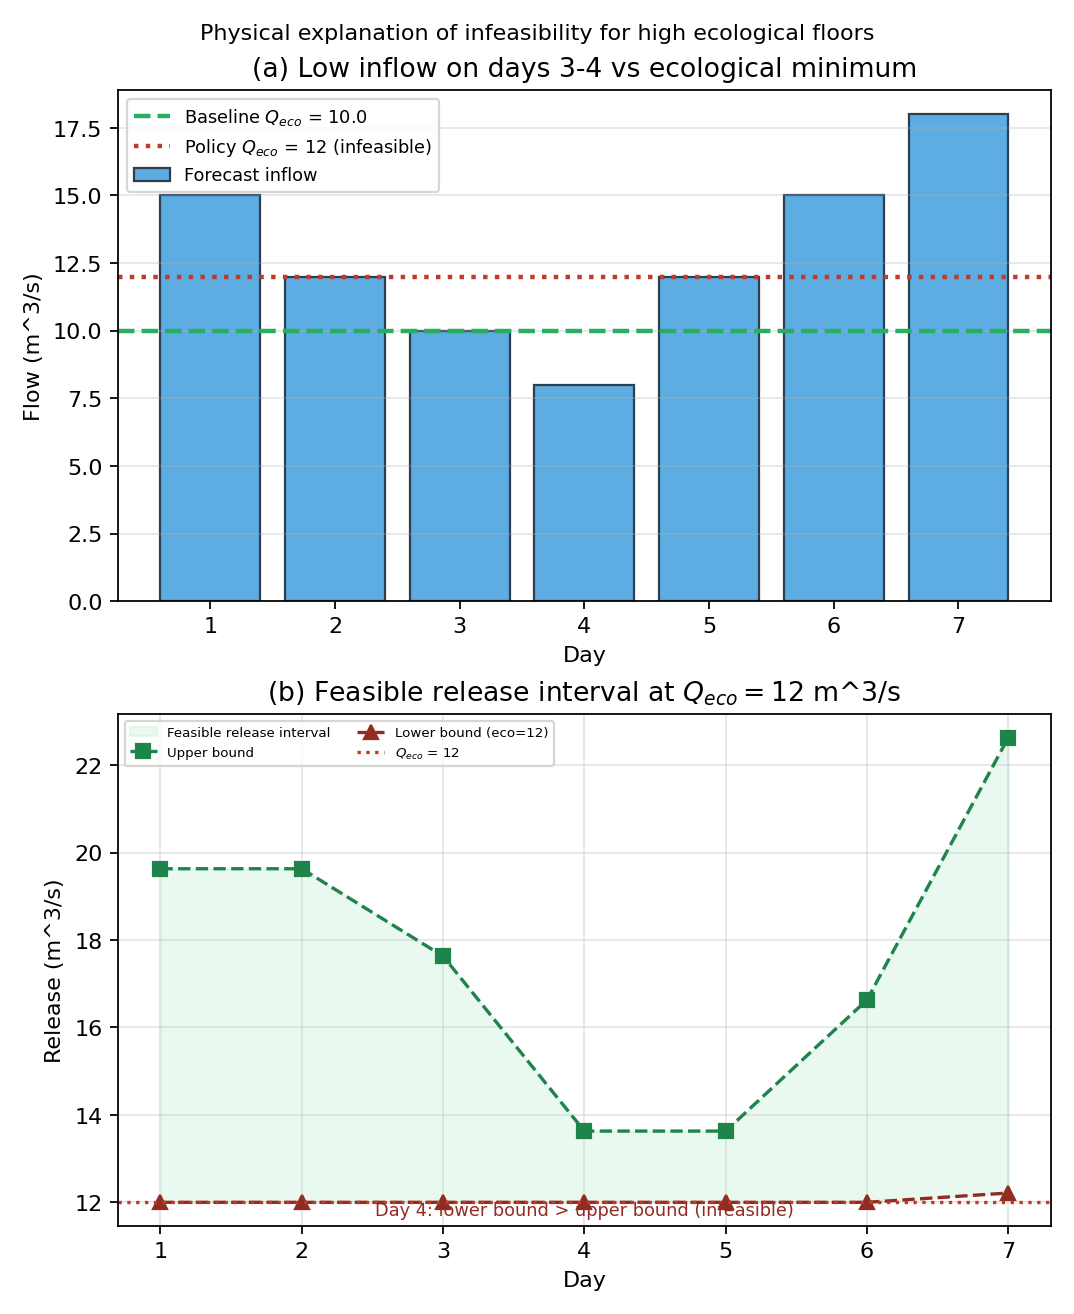
\includegraphics[width=\linewidth]{screenshots/infeasibility_explanation.png}
  \caption{Infeasibility when $Q_{\mathrm{eco}}\geq 12$~m$^3$/s: low inflow on days 3--4 and narrowing feasible release bounds.}
  \label{fig:infeasible}
\end{figure}

\textbf{Operational balance defended:} $Q_{\mathrm{eco}}=10$~m$^3$/s is the maximum ecological floor compatible with this drought inflow without violating storage; higher floors require inflow relief or policy revision.

%=============================================================================
\section{Part 5: Validation (10\%)}
%=============================================================================

\texttt{validation\_report.txt} includes seven sections: parameters, summary, day-by-day schedule, constraint margins, continuity check, solver comparison, head sensitivity.

\begin{table}[htbp]
  \centering
  \caption{Validation matrix.}
  \label{tab:valid}
  \begin{tabular}{@{}ll@{}}
    \toprule
    Check & Result \\
    \midrule
    Storage bounds & PASS (0 violations) \\
    Release bounds & PASS \\
    Mass balance & PASS ($<10^{-3}$~m$^3$) \\
    Eco deficit at $Q_{\mathrm{eco}}=10$ & 0 \\
    Revenue recomputation & PASS \\
    \bottomrule
  \end{tabular}
\end{table}

\begin{figure}[htbp]
  \centering
  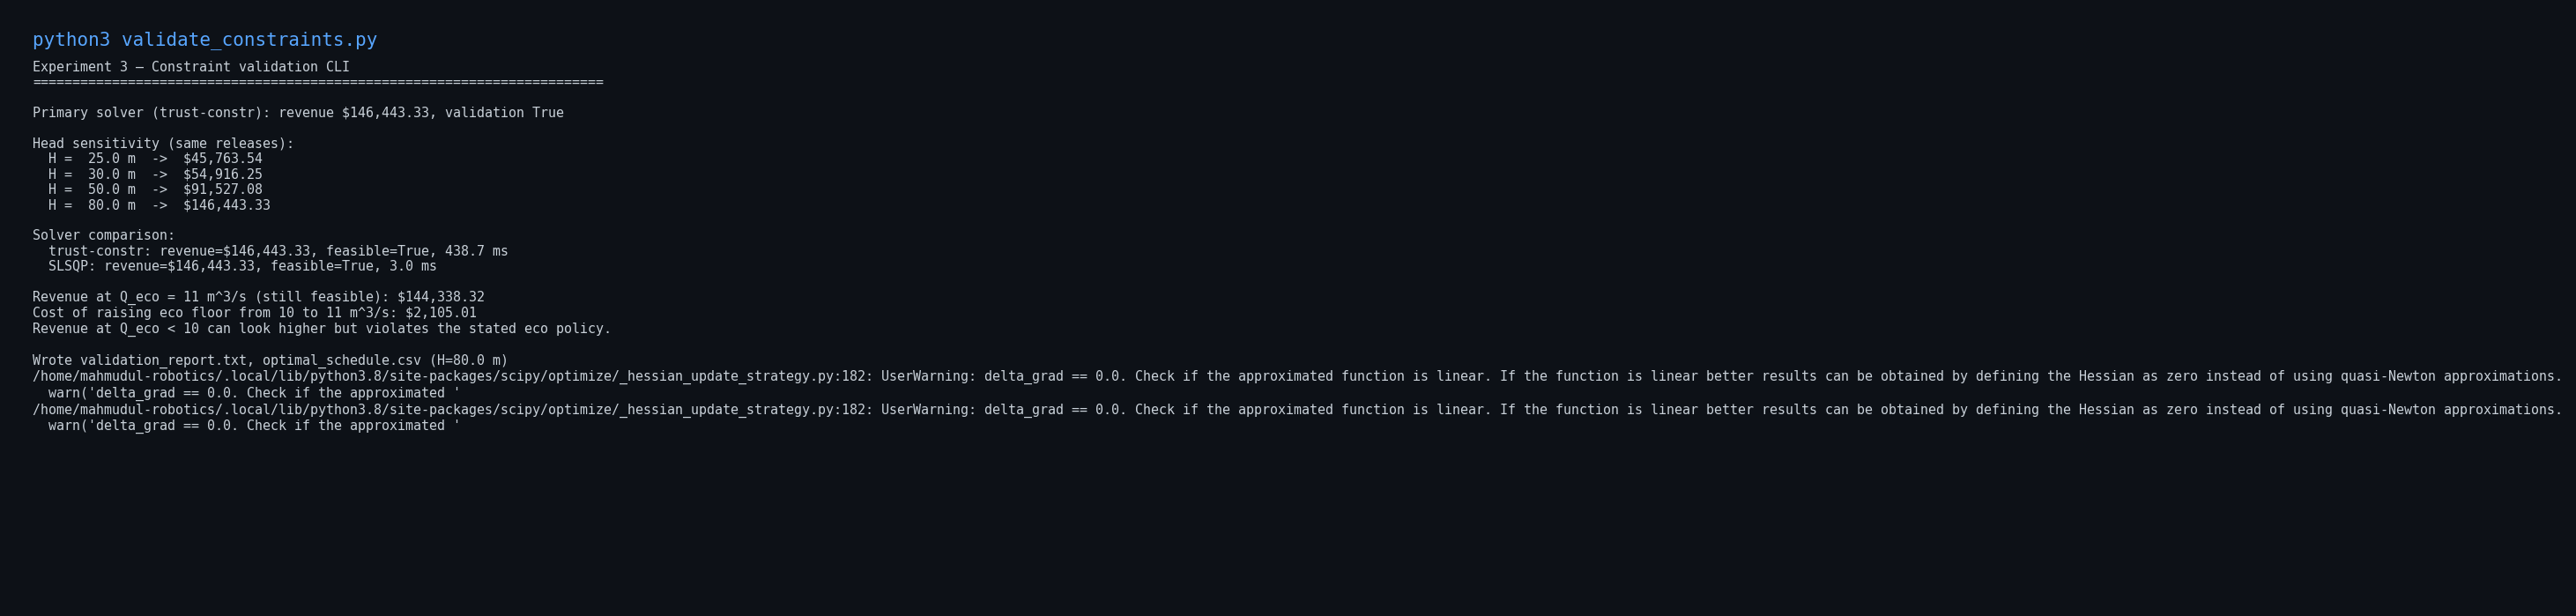
\includegraphics[width=\linewidth]{screenshots/experiment3_validation.png}
  \caption{Validation CLI: \texttt{validate\_constraints.py} (solver compare + head table).}
  \label{fig:validation}
\end{figure}

%=============================================================================
\section{Discussion and Lessons}
%=============================================================================

Joint horizon optimization with a feasible $x_0$ is essential; myopic daily maximization can violate future storage bounds. Trade-off sweeps must use the \textbf{true} policy floor in release bounds. Revenue magnitude follows head; constraints and schedule shape align with peers using $H\approx 30$~m. Figure~\ref{fig:storagebounds} provides immediate visual proof of feasibility; Figure~\ref{fig:infeasible} links infeasibility to hydrology on days 3--4.

\section{AI-Augmented Software Engineering}
\label{sec:ai-eng}

\subsection{Swiss Cheese Model --- layered verification}
\begin{table}[htbp]
  \centering
  \caption{Verification layers (Experiment 3).}
  \label{tab:swiss3}
  \begin{tabular}{@{}ll@{}}
    \toprule
    Layer & Result \\
    \midrule
    Human formulation (\texttt{formulation.md}) & Written before solver code \\
    Unit + scenario tests & 20 pytest passed \\
    Physical constraints & Storage, eco, mass balance \\
    Validation CLI & \texttt{validate\_constraints.py} PASS \\
    Trade-off honesty & Infeasible $Q_{\mathrm{eco}}\ge 12$ flagged, not faked \\
    Drought scenario & Infeasible at 70\% inflow (documented) \\
    \bottomrule
  \end{tabular}
\end{table}

\subsection{Jagged Frontier --- AI mistake caught}
\textbf{AI output:} SLSQP alone converged to infeasible high-revenue schedules (storage below $V_{\min}$); trade-off sweep initially used an incorrect ecological lower bound.

\textbf{Detection:} \texttt{validate\_schedule()} violations; days 3--4 low inflow; scenario analysis marks drought infeasible.

\textbf{Human correction:} Feasible forward pass for $x_0$; \texttt{trust-constr}; true policy floor in release bounds; \texttt{scenario\_analysis.py} for drought/normal/wet.

\subsection{Tool evaluation (summary)}
Cursor Agent for implementation; DeepSeek/ChatGPT recommended for optimization math cross-check. \texttt{AGENTS.md} defines prohibited shortcuts (e.g.\ masking infeasibility).

\section{Reproducibility}
\label{sec:repro}

\textbf{Environment:} Python 3.8; \texttt{numpy}, \texttt{scipy}, \texttt{matplotlib}, \texttt{pandas}, \texttt{pytest} (see \texttt{requirements.txt}).

\textbf{Commands} (from \texttt{experiment3\_reservoir\_optimization/}):
\begin{verbatim}
pip install -r requirements.txt
python3 main.py
python3 validate_constraints.py
python3 tradeoff_analysis.py
pytest -v
python3 generate_report_figures.py
\end{verbatim}

\textbf{Outputs:} \texttt{optimal\_schedule.csv}, \texttt{validation\_report.txt}, \texttt{tradeoff\_analysis.png}, \texttt{storage\_bounds.png}, \texttt{infeasibility\_explanation.png}, \texttt{solver\_comparison.csv}.

\section{Conclusion}
All Experiment~3 deliverables are complete and strengthened per rubric section: \texttt{formulation.md}, \texttt{reservoir\_optimize.py}, \texttt{optimal\_schedule.csv}, \texttt{tradeoff\_analysis.png}, \texttt{validation\_report.txt}, \texttt{prompt\_log.md}, plus \texttt{validate\_constraints.py}, \texttt{tradeoff\_analysis.py}, and 18 pytest cases.

\appendix
\section{Formulation excerpt}
\filebox{\texttt{formulation.md} (opening)}{formulation.md}
\section{Validation CLI}
\filebox{\texttt{validate\_constraints.py}}{validate_constraints.py}
\section{Prompt log}
\filebox{\texttt{prompt\_log.md}}{prompt_log.md}

\end{document}
